%%%%%%%%%%%%%%%%%%%%%%%%%%
%                          %
% ----- INTRODUCTION ----- %
%                          %
%%%%%%%%%%%%%%%%%%%%%%%%%%


%
%
% WORDCLOUD
%
%

\section{Wordcloud}

	\subsection{Concept}

		Le wordcloud montre à l'utilisateur la liste des mots qu'il lit le plus fréquemment. Le visualisation est un amassage de mots de différentes tailles, placés d'une manière aléatoire sur un rectangle. Les mots les plus lus ont une taille plus grande afin d'attirer l'attention de l'utilisateur.

		Cette visualisation cherche à donner très rapidement une impression générale des thèmes que l'utilisateur parcourt lors de sa navigation.

		\begin{figure}[!h]
			\centering
			\subfloat[Maquette initiale de la vue]{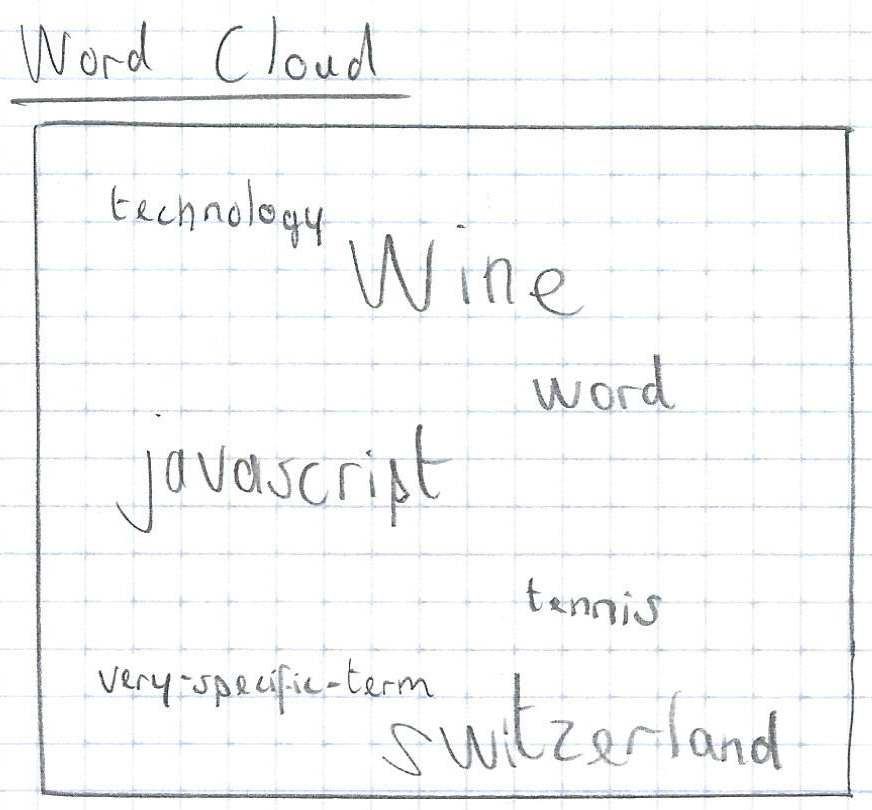
\includegraphics[width=0.33\textwidth,valign=t]{images/design/pages/wordcloud_mockup}}
			\subfloat[Exemple de résultat final]{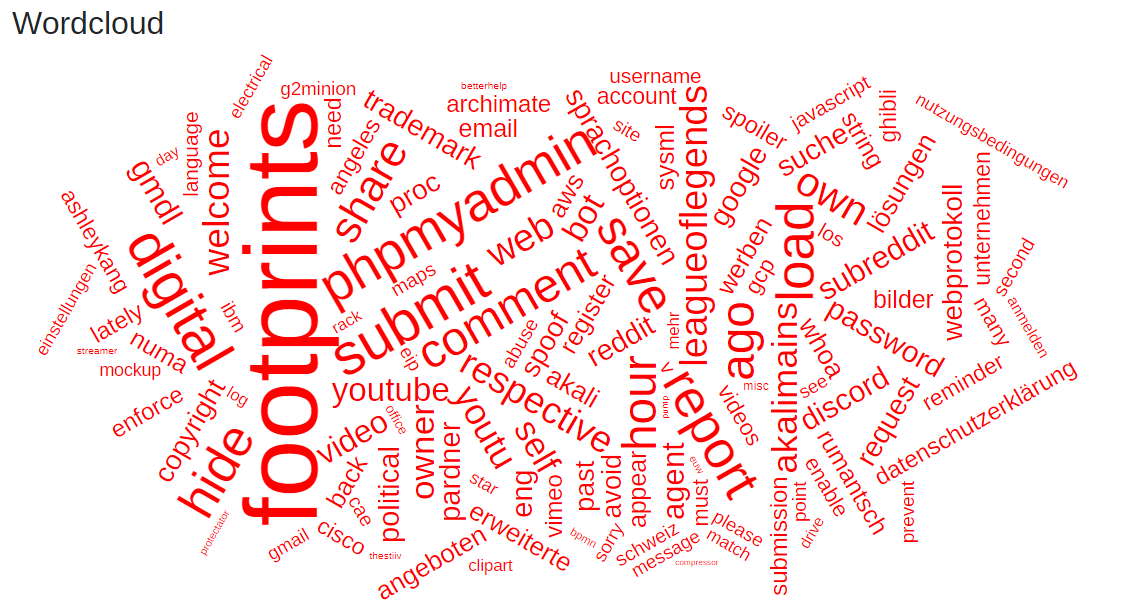
\includegraphics[width=0.66\textwidth,valign=t]{images/design/pages/wordcloud_final}}
			\caption{Maquette initiale et résultat final de la vue Wordcloud}
			\label{wordcloud_images}
		\end{figure}

		La figure~\ref{wordcloud_images} montre la différence entre la vue imaginée initialement et le résultat final.

	\subsection{Données}

		\subsubsection{Sources}

			Les données source servant à constituer cette visualisation sont :
			\begin{description}
				\item[Temps de visualisation] : Temps de visualisation total de chaque page. Ces données sont stockées dans la table \texttt{pagewatch} (figure \ref{table-content}).
				\item[Poids TF-IDF] : Poids final selon l'algorithme TF-IDF de chaque mot. Ces données sont stockées dans la table \texttt{computed\_tfidf} (figure \ref{table-computed-tfidf}).
			\end{description}
		\subsubsection{Algorithme}

			Afin de déterminer quels sont les mots affichés ainsi que leur taille sur la visualisation, on assigne un "poids" à chaque mot.

			La figure~\ref{wordcloud_algo} illustre le fonctionnement de l'algorithme utilisé :
			\begin{description}
				\item[A] On calcule le poids de chaque mot dans chaque document en effectuant la méthode de TF-IDF.

				\item[B] On effectue la somme du temps que l'utilisateur a passé à regarder chaque page visitée. Cette opération est effectuée sur le serveur, et l'interface obtient ce résultat en appelant l'endpoint \texttt{/api/mostWatchedSites} du serveur. Le résultat de cet appel est une liste de l'ensemble des pages web visitées, comprenant entre autres pour chaque page : 
				\begin{itemize}
					\item Son URL
					\item Le temps total de visite, en secondes
					\item Une liste des mots les plus significatifs selon TF-IDF ainsi que leur poids TF-IDF (normalisé entre 0 et 1)
				\end{itemize}
				
				On initialise un dictionnaire qui va contenir le poids de chaque mot.

				\item[C] Pour chaque page web, on multiplie l'indice TF-IDF de chaque mot avec le temps de visualisation de la page. On additionne ce résultat au poids actuel du mot.
				
				Une fois tous les mots de toutes les pages web traités, nous sommes en possession d'un dictionnaire nous indiquant le poids final de chaque mot. Ce poids est donc égal à la somme de l'indice TF-IDF du mot sur chaque page multiplié par le temps de visite sur cette page.
				
				\item[D] On trie les mots par leur poids final, et on ne conserve que les 200 premiers. Il s'agira des 200 mots présents sur le wordcloud.
				
				Pour chacun des 200 mots, leur taille sur le Wordcloud est égale à leur poids final.
			\end{description}

			\begin{figure}[!h]
				\centering
				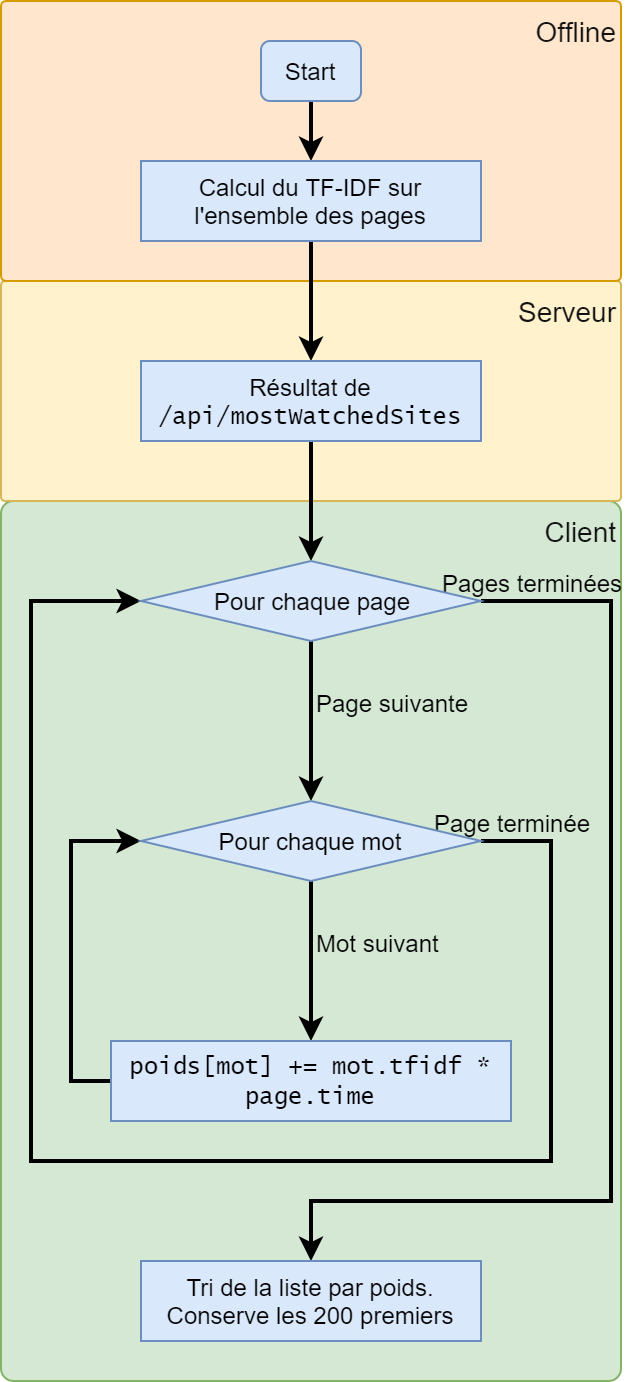
\includegraphics[height=1\textwidth]{images/design/pages/wordcloud_algo}
				\caption{Algorithme utilisé pour le Wordcloud}
				\label{wordcloud_algo}
			\end{figure}

	\subsection{Implémentation}

		\subsubsection{Serveur}

			La somme du temps de visualisation des pages est calculée en direct par une commande MySQL, elle est donc constamment à jour.

			Le poids TF-IDF de chaque mot est stocké dans la base de données, mais n'est pas constamment rafraîchi. L'opération de calcul des poids TF-IDF est une opération ponctuelle qui doit être lancée sur l'entièreté de la base de données par l'administrateur. Cette opération ne nécessite cependant pas de redémarrage du serveur.

			La concaténation de ces résultats (ainsi que certains autres qui ne sont pas utilisés par cette visualisation) est servie par l'endpoint \texttt{/api/mostWatchedSites} dans une liste en JSON.

		\subsubsection{Interface}

			La page va s'occuper d'agréger les résultats reçus du serveur. Ensuite, elle utilise les librairies \texttt{d3-cloud} ainsi que \texttt{d3} pour générer la visualisation du Wordcloud.

\clearpage

%
%
% TOPICS LIST
%
%

\section{Topics List}

	\subsection{Concept}

		Le "Topics List" cherche à rassembler les mots en thèmes, et montre d'une manière plus synthétique les thèmes estimés que l'utilisateur parcourt fréquamment. À chaque thème est lié un ou plusieurs mots, qui reprèsentent le thème d'une manière générale. Chaque cercle du graphe représente soit un thème, soit un mot.

		Le but de cette visualisation est de montrer que nous pouvons déduire des thèmes et ainsi montrer un traitement plus fin des intérêts de l'utilisateur, que simplement additionner une liste de mots. Dans le marketing, les thèmes découverts pourraient être utilisés pour labelliser les utilisateurs à qui faire apparaître une publicité.

		\begin{figure}[!h]
			\centering
			\subfloat[Maquette initiale de la vue]{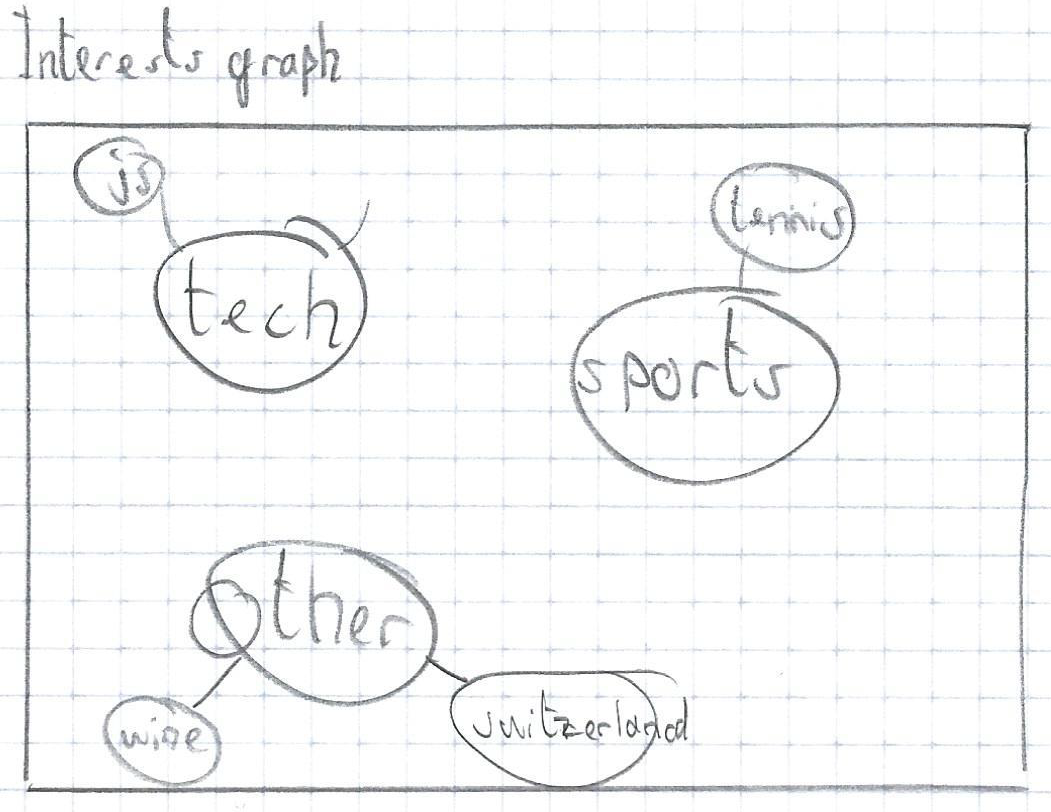
\includegraphics[width=0.33\textwidth,valign=t]{images/design/pages/topics_mockup}}
			\subfloat[Exemple de résultat final]{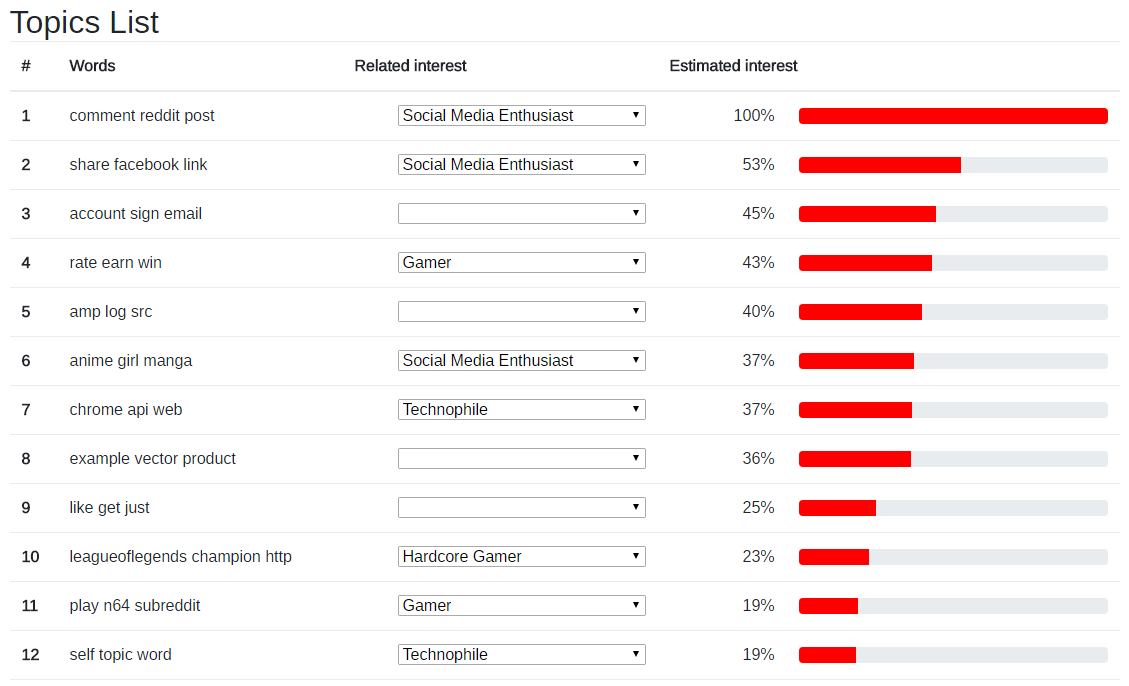
\includegraphics[width=0.66\textwidth,valign=t]{images/design/pages/topics_final}}
			\caption{Maquette initiale et résultat final de la vue Wordcloud}
			\label{topics_images}
		\end{figure}

		La figure~\ref{topics_images} montre la différence entre la vue imaginée et le résultat final. On note ici que le principe même de la vue ainsi que son nom sont différents qu'initialement.

	\subsection{Données}

		\subsubsection{Sources}

			Les données source servant à constituer cette visualisation sont :
			\begin{description}
				\item[Temps de visualisation] : Temps de visualisation total de chaque page. Ces données sont stockées dans la table \texttt{pagewatch} (figure \ref{table-content}).
				\item[Topics LDA] : Liste des topics générés par le modèle LDA. Ces données sont stockées dans la table \texttt{lda\_topics} (figure \ref{table-lda-topics}).
				\item[Topics par page] : Liste pré-caluclée des topics trouvés pour chaque page. Ces données sont stockées dans la table \texttt{current\_url\_topics} (figure \ref{table-current-url-topics}).
				\item[Intérêts utilisateur] : Liste des intérêts renseignés par l'utilisateur. Ces données sont stockées dans la table \texttt{user\_interests} (figure \ref{table-user-interests}).
				\item[Correspondances topic-intrêt] : Liste des correspondances entre topic et intérêt renseignés par l'utilisateur. Ces données sont stockées dans la table \texttt{current\_user\_tags} (figure \ref{table-current-user-tags}).
			\end{description}

		\subsubsection{Algorithme}

			Afin de déterminer quels sont les topics affichés ainsi que leur intérêt estimé, on assigne un "score" à chaque topic pour l'utilisateur.

			L'algorithme suivant, illustré par la figure~\ref{topics_algo}, est appliqué aux données sources :
			\begin{description}
				\item[A] On entraîne un modèle LDA avec un nombre défini de topics (typiquement 100) sur le contenu de l'ensemble des pages web, une page web représentant un document.
				
				Une fois le modèle LDA entraîné, on lui demande la liste des 100 topics générés par leur représentation en 5 mots. Cette liste de topics est enregistrée dans la base de données.

				\item[B] Pour chaque page enregistrée, on demande au modèle LDA quels sont les 5 topics les plus probables avec leur score de probabilité. Ces informations sont également enregistrées dans la base de données. Jusqu'ici, toutes ces opérations sont donc déjà calculées et se font avant le lancement du serveur. Elles ne sont pas mises à jour en temps réel.
				
				\item[C] On effectue la somme du temps que l'utilisateur a passé à regarder chaque page visitée. Cette opération est effectuée sur le serveur, et l'interface obtient ce résultat en appelant l'endpoint \texttt{/api/mostWatchedSites} du serveur. Le résultat de cet appel est une liste de l'ensemble des pages web visitées, comprenant entre autres pour chaque page : 
				\begin{itemize}
					\item Son URL
					\item Le temps total de visite, en secondes
					\item Une liste des topics les plus significatifs selon le modèle LDA ainsi que leur probabilité
				\end{itemize}

				\item[D] L'endpoint \texttt{/api/allTopics} renvoie la liste des topics générés par LDA ainsi que leur numéro d'identifiant.

				\item[E] L'endpoint \texttt{/api/getCurrentTags} renvoie la liste des associations que l'utilisateur a crée pour le modèle LDA courant. Il s'agit d'une liste de couples topicId $\longleftrightarrow$ interestId.

				\item[F] L'endpoint \texttt{/api/interestsList} renvoie la liste des 101 intérêts globaux à tous les utilisateurs.

				\item[G] On initialise un dictionnaire qui va contenir le score de chaque topic.
				
				Pour chaque page web, on multiplie la probabilité de chaque topic LDA avec le temps de visualisation de la page. On additionne ce résultat au score actuel du topic.
				
				Une fois tous les topics de toutes les pages web traités, nous sommes en possession d'un dictionnaire nous indiquant le score final de chaque topics. Ce score est donc égal à la somme de la probabilité du topic sur chaque page multiplié par le temps de visite sur cette page.
				
				\item[H] On trie les topics par leur score final, et on ne conserve que les 20 premiers. Il s'agira des 20 topics présents sur la page.

				\item[I] On sélectionne les centres d'intérêt de l'utilisateur, ainsi que les associations qu'il a déjà crée pour le modèle LDA actuel. On ajoute les associations aux topics de l'interface.
			\end{description}

			\begin{figure}[!h]
				\centering
				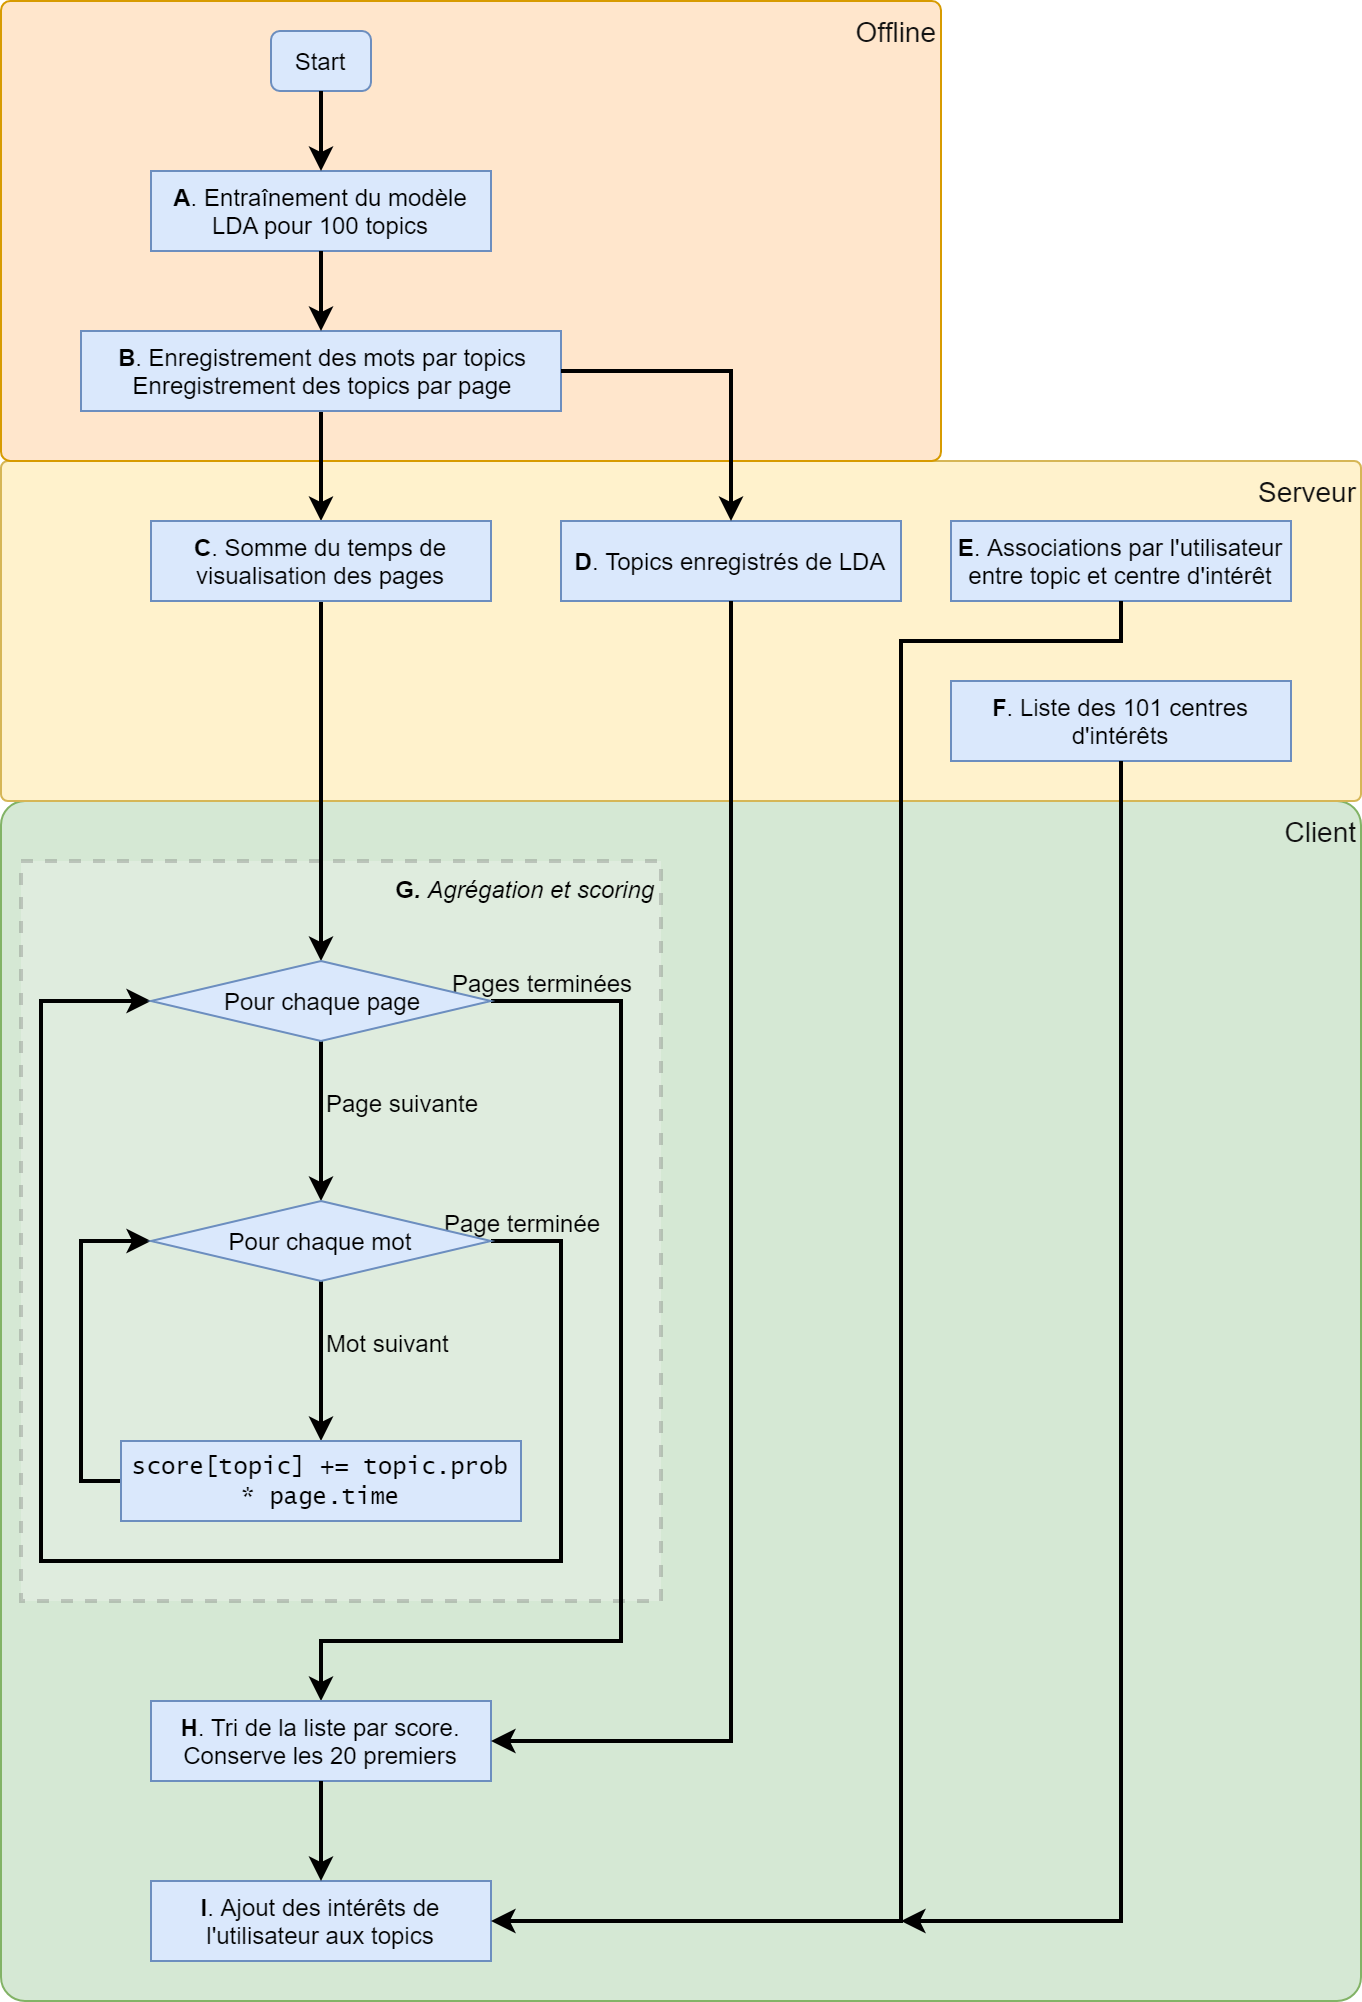
\includegraphics[height=1.35\textwidth]{images/design/pages/topics_algo}
				\caption{Algorithme utilisé pour le Topics List}
				\label{topics_algo}
			\end{figure}

	\subsection{Implémentation}

		\subsubsection{Serveur}

			La somme du temps de visualisation des pages est calculée en direct par une commande MySQL, elle est donc constamment à jour.

			Le modèle LDA est enregistré sur le disque local, et les résultats pré-calculés sont stocké dans la base de données, tout ceci n'est donc pas constamment rafraîchi. L'opération d'entraînement du modèle LDA est une opération ponctuelle qui doit être lancée sur l'entièreté de la base de données par l'administrateur. Cette opération nécessite le redémarrage du serveur, car de nombreuses mesures temporaires sont touchées.

			La concaténation de ces résultats (ainsi que certains autres qui ne sont pas utilisés par cette visualisation) est servie par l'endpoint \texttt{/api/mostWatchedSites} dans une liste en JSON. L'endpoint \texttt{/api/interestsList} est utilisé pour afficher le nom des centres d'intérêts, et l'endpoint \texttt{/api/getCurrentTags} donne l'ensemble des associations que l'utilisateur a crée entre ses centres d'intérêts, et les topics LDA actuels.

		\subsubsection{Interface}

			La page va s'occuper d'agréger les résultats reçus du serveur. La liste est ensuite générée sous forme d'un tableau HTML en passant par un composant Vue personnalisé. Les barres d'intérêt sont des éléments \texttt{progressbar} venant de Bootstrap.

\clearpage

%
%
% MOST WATCHED
%
%

\section{Most Watched}

	\subsection{Concept}

		Les pages "Most Watched" et "Most Visited" montrent deux informations, mais sous une forme semblable. Ces pages affichent quelles pages web et les domaines que l'utilisateur a visité le plus. Plus précisément, "Most Watched" s'intéresse au temps réel passé à lire chaque page, et "Most Visited" s'intéresse au nombre d'ouvertures de l'URL.

		Le but est ici de faire prendre conscience à l'utilisateur qu'il est possible de se rendre compte de son activité une page web, et un grand nombre d'ouvertures d'un lien ne veut pas forcément dire un grand intérêt pour cette page.

		On profite également de cet espace pour afficher les mots relatifs aux pages web qui ont le plus d'intérêt, afin de montrer qu'il est possible de déterminer quels sont les mots importants d'une page web simplement en la comparant au contenu des autres pages.

		La figure~\ref{mostwatched_images} montre la différence entre la vue imaginée et le résultat final.

		\begin{figure}[!h]
			\centering
			\subfloat[Maquette initiale de la vue]{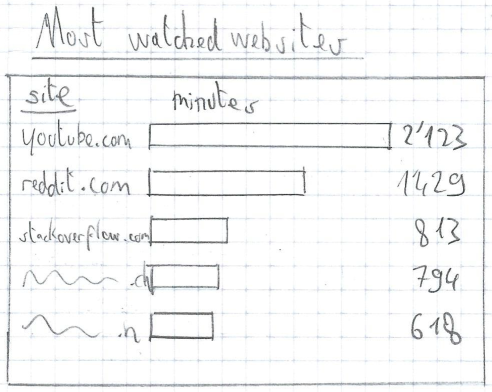
\includegraphics[width=0.33\textwidth,valign=t]{images/design/pages/mostwatched_mockup}}
			\subfloat[Exemple de résultat final]{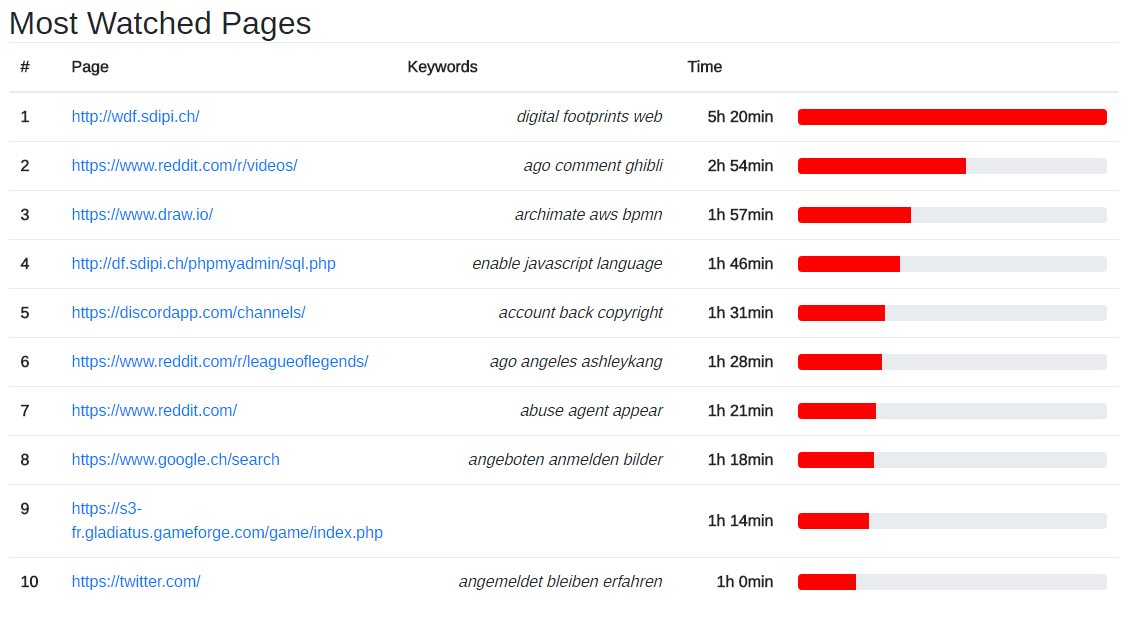
\includegraphics[width=0.66\textwidth,valign=t]{images/design/pages/mostwatched_final}}
			\caption{Maquette initiale et résultat final de la vue Most Watched}
			\label{mostwatched_images}
		\end{figure}

		Comme certaines pages web demandent une connexion pour être visualisées, par exemple la page d'accueil de \url{https://www.facebook.com}, nous omettons volontairement une liste de pages web dans ce classement, car nous n'avons pas d'informations intéressante sur leur contenu à montrer. En effet, nous ne téléchargeons volontairement pas de copie de la page vue par l'utilisateur pour des questions de protection de données privées. Notre serveur télécharge la version publique de l'URL visitée par l'utilisateur pour en déterminer son contenu. Ainsi, il ne fait pas sens d'analyser le contenu des pages générées dynamiquement par l'utilisateur.

	\subsection{Données}

		\subsubsection{Sources}

			Les données source servant à constituer cette visualisation sont :
			\begin{description}
				\item[Temps de visualisation] : Temps de visualisation total de chaque page. Ces données sont stockées dans la table \texttt{pagewatch} (figure \ref{table-content}).
				\item[Nombre de visites] : Nombre total d'ouvertures de chaque URL. Ces données sont stockées dans la table \texttt{pageviews} (figure \ref{table-pageviews}).
				\item[Poids TF-IDF] : Poids final selon l'algorithme TF-IDF de chaque mot. Ces données sont stockées dans la table \texttt{computed\_tfidf} (figure \ref{table-computed-tfidf}).
			\end{description}

		\subsubsection{Algorithme}

		Afin de déterminer quels sont les pages et les domaines affichés, on demande au serveur la liste triée des URLs les plus regardées et ouvertes.

			L'algorithme suivant, illustré par la figure~\ref{mostwatched_algo}, est appliqué aux données sources :
			\begin{description}
				\item[A] On calcule le poids de chaque mot dans chaque document en effectuant la méthode de TF-IDF.

				\item[B] On effectue la somme du temps que l'utilisateur a passé à regarder chaque page visitée. Cette opération est effectuée sur le serveur, et l'interface obtient ce résultat en appelant l'endpoint \texttt{/api/mostWatchedSites} du serveur. Le résultat de cet appel est une liste de l'ensemble des pages web regardées, comprenant entre autres pour chaque page : 
				\begin{itemize}
					\item Son URL
					\item Le temps total de visite, en secondes
					\item Une liste des mots les plus significatifs selon TF-IDF ainsi que leur poids TF-IDF (normalisé entre 0 et 1)
				\end{itemize}

				\item[C] On effectue la somme du nombre d'ouvertures de chaque page visitée. Cette opération est effectuée sur le serveur, et l'interface obtient ce résultat en appelant l'endpoint \texttt{/api/mostWatchedSites} du serveur. Le résultat de cet appel est une liste de l'ensemble des pages web visitées, comprenant entre autres pour chaque page : 
				\begin{itemize}
					\item Son URL
					\item Le nombre total d'ouvertures
					\item Une liste des mots les plus significatifs selon TF-IDF ainsi que leur poids TF-IDF (normalisé entre 0 et 1)
				\end{itemize}
				
				\item[D] Une fois la liste des pages les plus regardées obtenue, on ne conserve que les 10 premières d'entre-elles pour des raisons visuelles. Ces 10 premières pages sont alors affichées.

				\item[E] Ensuite, on cherche à agréger le temps de visualisation par domaine plutôt que par page, afin d'avoir une vue d'ensemble. On additionne donc le temps passé à regarder les pages d'un même domaine.

				\item[F] On trie la nouvelle liste de domaines crée par leur temps total de visualisation, et on ne garde également que les 10 premiers d'entre-eux pour les afficher.

				\item[G] On s'occupe ensuite du traitement du nombre d'ouvertures de chaque page. On ne conserve également que les 10 plus ouvertes d'entre-elles pour des raisons visuelles, elles sont alors affichées dans la liste.

				\item[H] Ensuite, on agrèger le nombre d'ouvertures par domaine plutôt que par page, afin d'avoir une vue d'ensemble. On additionne donc le temps passé à regarder les pages d'un même domaine.

				\item[I] On trie la nouvelle liste de domaines crée par leur temps total de visualisation, et on ne garde également que les 10 premiers d'entre-eux pour les afficher.
			\end{description}

			\begin{figure}[!h]
				\centering
				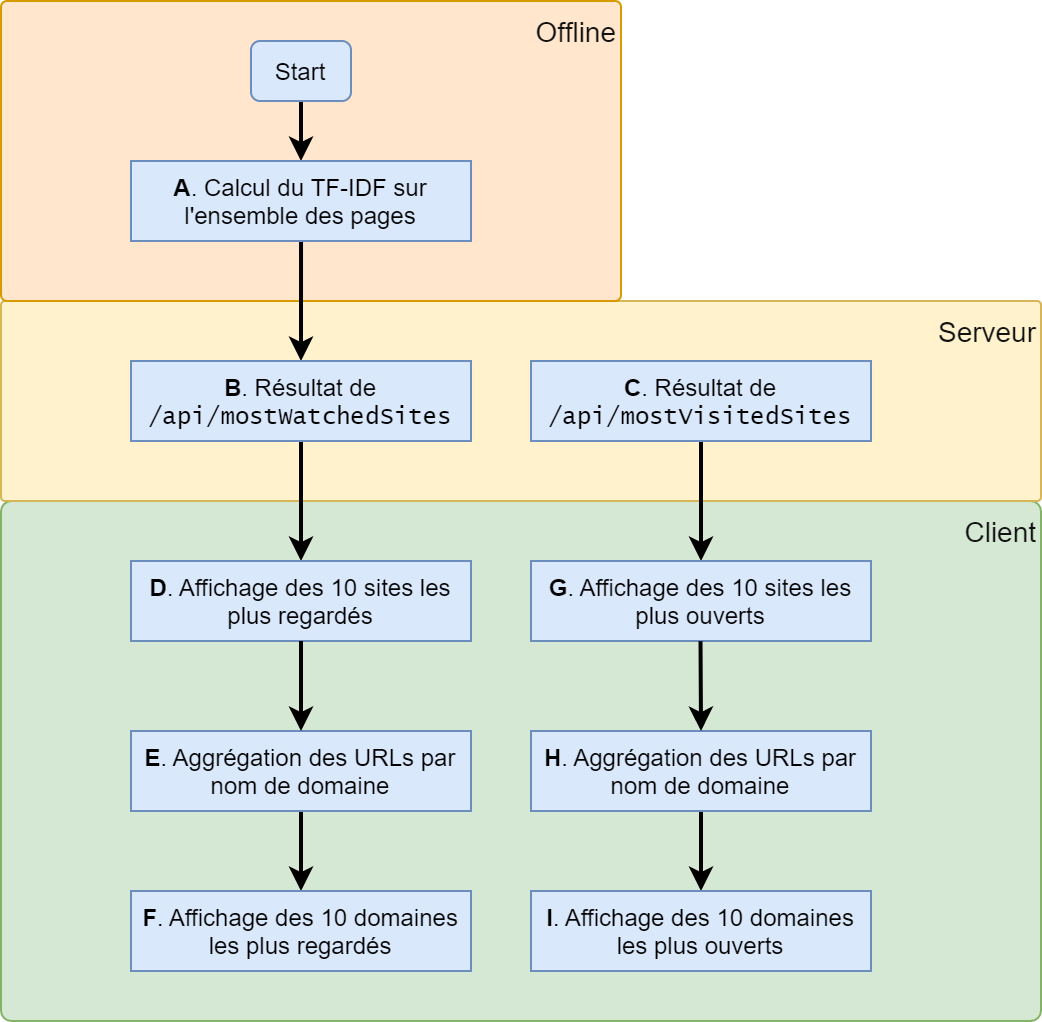
\includegraphics[height=0.8\textwidth]{images/design/pages/mostwatched_algo}
				\caption{Algorithme utilisé pour les pages "Most Watched" et "Most Visited"}
				\label{mostwatched_algo}
			\end{figure}

	\subsection{Implémentation}

		\subsubsection{Serveur}

			La somme du temps de visualisation des pages ainsi que du total d'ouvertues est calculée en direct par une commande MySQL, elle est donc constamment à jour.

			Le poids TF-IDF de chaque mot est stocké dans la base de données, mais n'est pas constamment rafraîchi. L'opération de calcul des poids TF-IDF est une opération ponctuelle qui doit être lancée sur l'entièreté de la base de données par l'administrateur. Cette opération ne nécessite cependant pas de redémarrage du serveur.

			La concaténation des résultats du temps total de visualisation ainsi que du nombre d'ouvertues est servi par respectivement l'endpoint \texttt{/api/mostWatchedSites}, et \texttt{/api/mostVisitedSites}.

		\subsubsection{Interface}

			La page va s'occuper d'agréger les résultats reçus du serveur. Chaque liste est ensuite générée sous forme d'un tableau HTML en passant par un composant Vue personnalisé. Les barres relatives à la quantité exprimée par chaque tableau ajoute un élément de comparaison visuel, et sont des éléments \texttt{progressbar} venant de Bootstrap.

\clearpage

%
%
% HISTORY
%
%

\section{History}

	\subsection{Concept}

		La page "History" permet de montrer à l'utilisateur la variation de ses habitudes au cours du temps durant lequel il a utilisé l'extension. Deux graphiques sont présents sur cette page : Le premier montre la tendence à visiter des pages relatées à certains topics, et l'autre montre la tendence dans la visite de pages contenant certains mots particuliers. Le but est ici de détecter d'éventuels intérêts passagers dans le temps.

		La figure~\ref{history_images} montre la différence entre la vue imaginée et le résultat final.

		\begin{figure}[!h]
			\centering
			\subfloat[Maquette initiale de la vue]{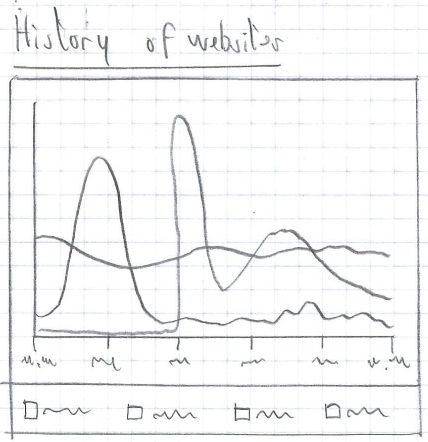
\includegraphics[width=0.3\textwidth,valign=t]{images/design/pages/history_mockup}}
			\subfloat[Exemple de résultat final]{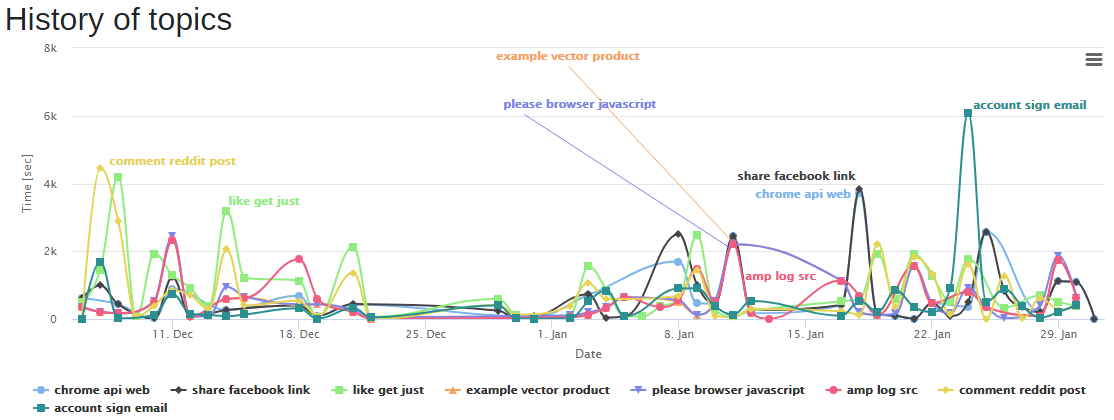
\includegraphics[width=0.7\textwidth,valign=t]{images/design/pages/history_final}}
			\caption{Maquette initiale et résultat final de la vue History}
			\label{history_images}
		\end{figure}

	\subsection{Données}

		\subsubsection{Sources}

			Les données source servant à constituer cette visualisation sont :
			\begin{description}
				\item[Temps de visualisation] : Temps de visualisation total de chaque page. Ces données sont stockées dans la table \texttt{pagewatch} (figure \ref{table-content}).
				\item[Historique de visualisation] : Temps passé par jour sur chaque URL. Les données non agrégées proviennent de la table \texttt{pageviews} (figure \ref{table-pagewatch}).
				\item[Poids TF-IDF] : Poids final selon l'algorithme TF-IDF de chaque mot. Ces données sont stockées dans la table \texttt{computed\_tfidf} (figure \ref{table-computed-tfidf}).
				\item[Topics LDA] : Liste des topics générés par le modèle LDA. Ces données sont stockées dans la table \texttt{lda\_topics} (figure \ref{table-lda-topics}).
			\end{description}

		\subsubsection{Algorithme}

			Afin de déterminer quels sont les topics et les mots cumulant le plus d'intérêt, il est nécessaire de disposer de plusieurs sources de données et de les assembler afin d'arriver au résultat voulu. Ceci se fait en plusieurs étapes, distribuées entre le serveur et client.

			L'algorithme suivant, illustré par la figure~\ref{history_algo}, est appliqué aux données sources :
			\begin{description}
				\item[A] On calcule le poids de chaque mot dans chaque document en effectuant la méthode de TF-IDF.

				\item[B] On entraîne un modèle LDA avec un nombre défini de topics (typiquement 100) sur le contenu de l'ensemble des pages web, une page web représentant un document.
				
				Une fois le modèle LDA entraîné, on lui demande la liste des 100 topics générés par leur représentation en 5 mots. Cette liste de topics est enregistrée dans la base de données.

				\item[C] Pour chaque page enregistrée, on demande au modèle LDA quels sont les 5 topics les plus probables avec leur score de probabilité. Ces informations sont également enregistrées dans la base de données. Jusqu'ici, toutes ces opérations sont donc déjà calculées et se font avant le lancement du serveur. Elles ne sont pas mises à jour en temps réel.

				\item[D] On demande à la base de données de grouper le temps de visionnage (en secondes) en une somme par jour et par URL différente. Ceci se fait au travers d'une commande MySQL, et est calculé en temps réel.

				\item[E] Le résultat de l'étape précédente est disponible via l'endpoint\\
				\texttt{/api/historySites}.

				\item[F] On effectue la somme du temps que l'utilisateur a passé à regarder chaque page visitée. L'interface obtient ce résultat en appelant l'endpoint\\
				\texttt{/api/mostWatchedSites} du serveur. Le résultat de cet appel est une liste de l'ensemble des pages web regardées, comprenant entre autres une liste des mots les plus significatifs selon TF-IDF ainsi que leur poids TF-IDF (normalisé entre 0 et 1) pour chaque page.
				
				\item[G] L'endpoint \texttt{/api/allTopics} renvoie la liste des topics générés par LDA ainsi que leur numéro d'identifiant.

				\item[H] On cherche à savoir quels sont les mots où lesquels l'utilisateur a montré le plus d'intérêt afin de les afficher sur le graphe. Pour ceci, on multiplie la valeur TF-IDF de chaque mot par le temps passé à visualiser la page. La somme de ce calcul sur toutes les pages va nous donner l'"intérêt" final de l'utilisateur pour un mot particulier. On ne gardera ici que les 8 mots avec le plus grand intérêt estimé.

				\item[I] Finalement, pour chacun des 8 mots retenus, on affiche leur intérêt journalier sur le deuxième graphique, "Words history".

				\item[J] On cherche à savoir quels sont les topics où lesquels l'utilisateur a montré le plus d'intérêt afin de les afficher sur le graphe.

				Voici ce que l'on effectue sur chaque page : Pour chaque topic où sa valeur selon le modèle LDA sur cette page est au-dessus de 0.1, on estie que la page parle de ce topic et on compte le temps passé à visualiser la page dans la valeur de ce topic pour la journée.

				Finalement, on somme le temps passé sur chaque "topic". Le résultat de ce calcul sur toutes les pages va nous donner l'"intérêt" final de l'utilisateur pour un topic particulier. On ne gardera ici que les 8 topics avec le plus grand intérêt estimé.

				\item[K] Finalement, pour chacun des 8 topics retenus, on affiche leur intérêt journalier (qui est la même somme que précédamment, mais agrégée par jour au lieu de toute la période) sur le premier graphique, "Topics history".
			\end{description}

			\begin{figure}[!h]
				\centering
				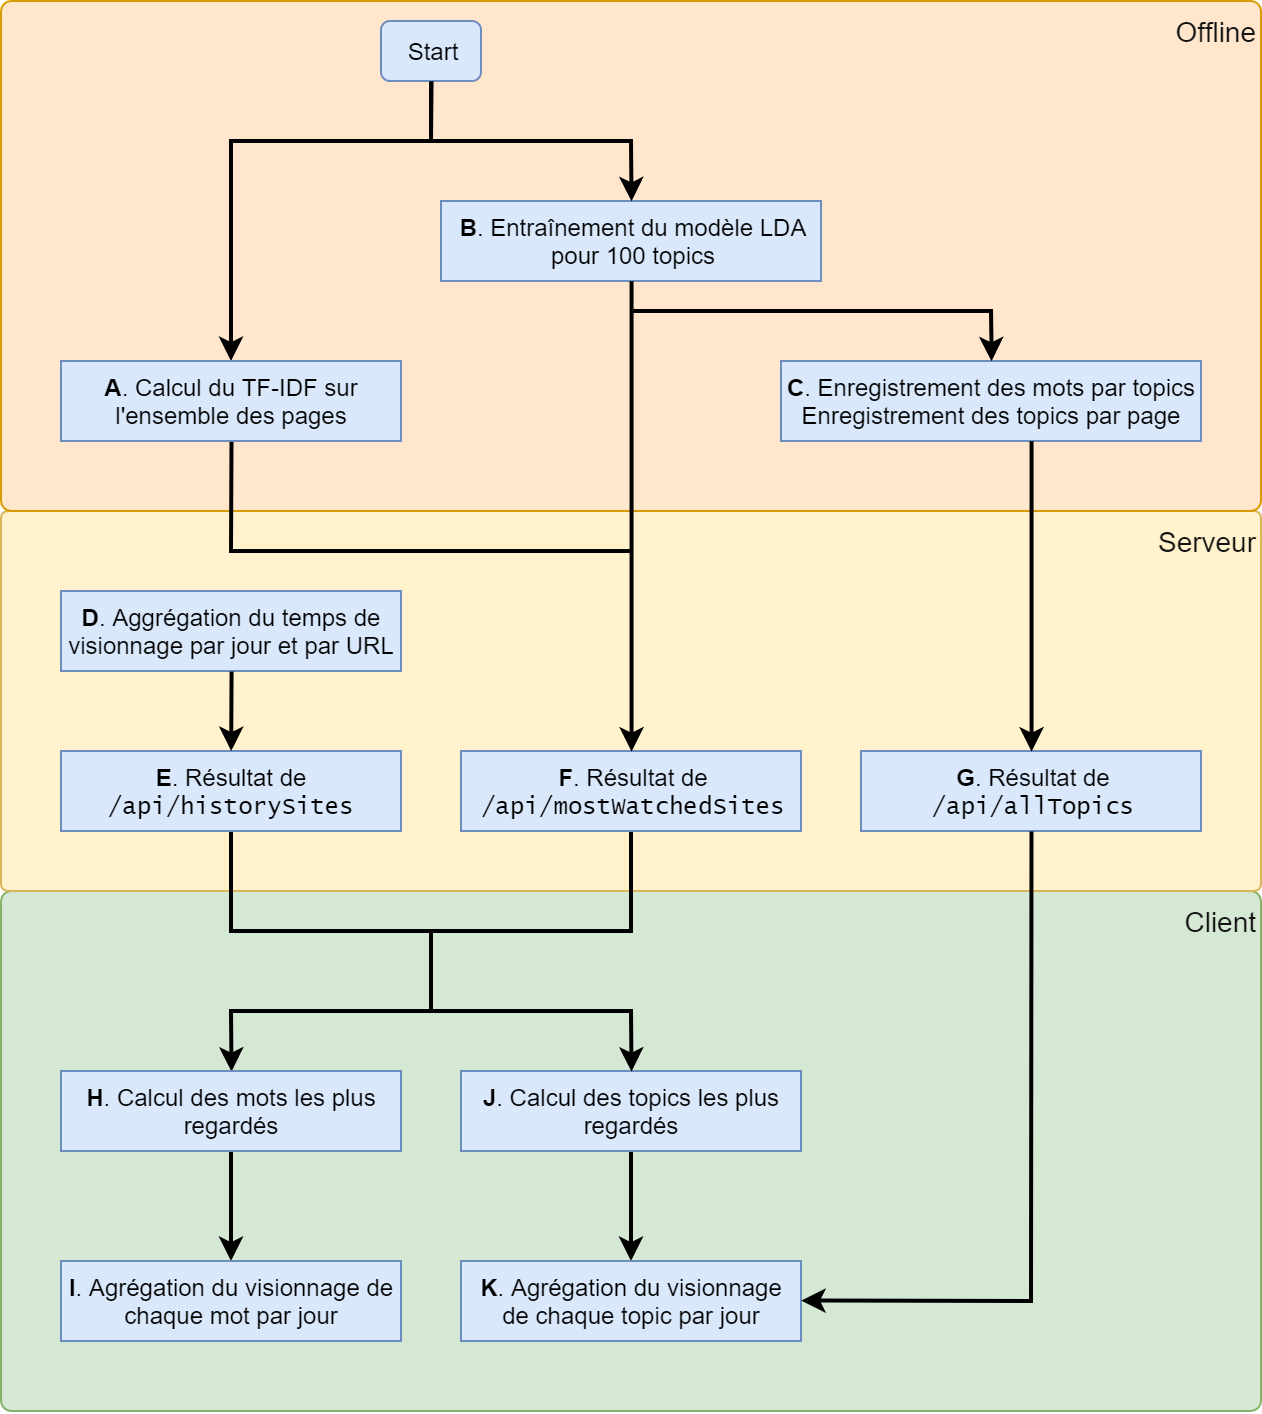
\includegraphics[height=1.15\textwidth]{images/design/pages/history_algo}
				\caption{Algorithme utilisé pour les graphiques de la page "History"}
				\label{history_algo}
			\end{figure}

	\subsection{Implémentation}

		\subsubsection{Serveur}

			La somme du temps de visualisation effectuée en temps réel sur le serveur est faire par une commande MySQL qui s'occupe également d'"arrondir" chaque date de visualisation d'une page à la journée (au lieu de la seconde près, qui est la granularité utilisée dans la base de données).

		\subsubsection{Interface}

			Les données sont finalement transformées dans un format compatible et passées à une instance configurée de la librairie HighCharts, qui génère la visualisation du graphique sur la page.

\section{Trackers}

	\subsection{Concept}

		La vue "Trackers" comporte deux pages et 

	\subsection{Données}

		\subsubsection{Sources}

		\subsubsection{Algorithme}

	\subsection{Implémentation}

		\subsubsection{Serveur}

		\subsubsection{Interface}

\section{Stats}

	\subsection{Concept}

	\subsection{Données}

		\subsubsection{Sources}

		\subsubsection{Algorithme}

	\subsection{Implémentation}

		\subsubsection{Serveur}

		\subsubsection{Interface}

\section{Settings}

	\subsection{Concept}

	\subsection{Données}

		\subsubsection{Sources}

		\subsubsection{Algorithme}

	\subsection{Implémentation}

		\subsubsection{Serveur}

		\subsubsection{Interface}